\documentclass[12pt]{report}
\usepackage{graphicx}
\graphicspath{ {./recursos/} }
\usepackage[spanish]{babel}
\usepackage[utf8]{inputenc}



%	\addtolength{\topmargin}{2cm}
%    \addtolength{\textheight}{1cm}

\renewcommand*\contentsname{Indice}

\begin{document}
% \thispagestyle{empty}

% \noindent\rule{\textwidth}{0.5pt}

\begin{minipage}{0.2\textwidth}
    
\includegraphics[width=\textwidth]{logo-ipn-guinda.png}
    \hspace{-\textwidth} % Desplaza la imagen a la izquierda
    \vspace{-\topskip}   % Desplaza la imagen hacia arriba
\end{minipage}%
\begin{minipage}{0.2\textwidth}
    \vspace{1.5cm} % Ajusta el espacio vertical según sea necesario
    \noindent\rule{10cm}{0.5pt}
\end{minipage}%

\begin{figure}[b]
\includegraphics[width=0.22\textwidth]{esime.png}
\end{figure} 

\begin{Huge}
	Control inteligente basado en navegación inercial para brazo robótico
\end{Huge}

\newpage

\tableofcontents

\newpage
\section*{Introduccion}

Los brazos robóticos articulados son sistemas mecánicos con articulaciones rotativas, diseñados para replicar funciones del brazo humano, incluyendo movimientos de rotación y alcance. Suelen tener una pieza en el extremo del robot llamado efector final (Fig. 1), que realiza la función del robot en el entorno (soldar, manipular objetos, etc.). Cada unión en las articulaciones representa un grado de libertad (DoF) [1].

\begin{figure}[htb]
	\centering
	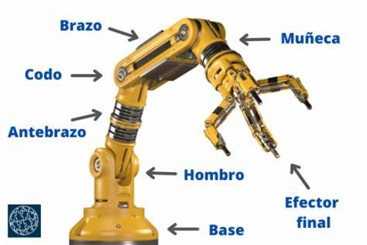
\includegraphics[scale=0.6]{brazo.jpg}
	\caption{Partes de un brazo robótico articulado de 3 DoF}
\end{figure}

Sistemas Eléctricos de Potencia Computarizada (SEPDC) es una empresa mexicana que se dedica a fabricar la serie Kaab (Fig. 2) de Controladores Lógicos Programables (PLC), computadoras especializadas para la automatización industrial (tienen inmunidad al ruido eléctrico y resistencia a la vibración y al impacto). Cada uno de ellos puede ser operado de forma remota a través de un software llamado SettDev. Dichos PLCs pueden ser empleados para controlar sistemas críticos.

\begin{figure}[htb]
	\centering
	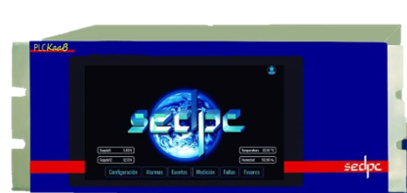
\includegraphics[scale=1]{plckaab.png}
	\caption{PLC-Kaab fabricado por SEDPC}
\end{figure}

\newpage
\section*{Planteamiento del problema}

Los brazos robóticos se han introducido rápidamente en la industria, sin embargo, aún existen desafíos para posicionar de manera precisa el brazo robótico que dificultan su introducción en industrias como la textil, sobre todo cuando dicho posicionamiento tiene que realizarse de manera autónoma [2].
\newline\newline\newline
Ubicar las articulaciones de un brazo para llegar a una posición deseada es un problema clásico de la robótica llamado cinemática inversa. Existen métodos algebraicos, geométricos e iterativos para resolverlo, sin embargo, dependen de la cantidad de grados de libertad del robot, además de que consumen una gran cantidad de recursos computacionales, lo que dificulta su uso en un sistema crítico [3].

\newpage
\section*{Objetivo general}

Desarrollar e implementar un sistema crítico de control, por medio de una Raspberry Pi, sensores inerciales y una red neuronal entrenada con aprendizaje no supervisado, para controlar la posición del efector final de un brazo robótico.

\newpage
\section*{Objetivos específicos}
\begin{itemize}
	
\item Desarrollar e implementar un programa en C++, utilizando los ángulos de inclinación en los tres ejes obtenidos por los sensores MPU6050, para determinar la posición del sensor en el extremo de la ortesis de brazo.

\item Implementar la comunicación entre la Raspberry Pi y el software SettDev por medio de sockets TCP en C++ y C\# para enviar los ángulos de inclinación calculados al software, para poder guardar los datos y permitir reproducirlos en la simulación en 3D de un brazo robótico.

\item Desarrollar e implementar una interfaz gráfica de usuario utilizando una pantalla táctil por medio del framework Qt para visualizar la cinemática inversa del brazo robótico a controlar.

\item Desarrollar e implementar en SettDev la comunicación entre el módulo del brazo robótico en 3D y el PLC por medio de sockets UDP en C\# para enviar los ángulos de inclinación al controlador y reproducir los ángulos de inclinación en los servomotores posicionales.

\item Implementar un sistema de inferencia neuro-difuso adaptativo (red neuronal ANFIS) utilizando C++ para resolver el problema de la cinemática inversa del brazo.

\item Desarrollar e implementar un algoritmo de aprendizaje no supervisado utilizando C++ para entrenar la red neuronal.

\end{itemize}
\newpage
\section*{Justificacion}

El sistema permitirá implementar un nuevo método para resolver la cinemática directa de forma trigonométrica a través de la navegación inercial, además de implementar un método que no dependa de la cantidad de grados de libertad del robot. Asimismo, será una aplicación práctica de las investigaciones previas a este trabajo sobre redes neuronales para el control de un brazo robótico.

\newpage
\section*{Estado del arte}

\newpage
\section*{Marco teorico}

\subsection*{Raspberry Pi 3 B+}
\begin{itemize}

	\item Funciona con un sistema operativo basado en la arquitectura ARM.
	
	\item Módulo Wi-Fi de banda dual de 2,4 y 5 GHz.
	
	\item 40 pines Entrada/Salida de Propósito General (GPIO)
	
	\item Salidas de 3.3 y 5 V, buses I²C, SPI
	
\end{itemize}

\begin{figure}[htb]
	\centering
	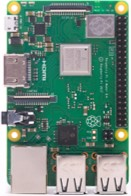
\includegraphics[scale=0.5]{raspberrypi.jpg}
	\caption{Raspberry Pi 3 B+}
\end{figure}

\subsection*{Qt}
\begin{itemize}
	
	\item Optimizada para aplicaciones con interfaces gráficas en sistemas embebidos.
	
	\item Soporte para C++
	
	\item Utiliza el lenguaje declarativo QML para programar la interfaz
	
\end{itemize}

\begin{figure}[htb]
	\centering
	
\includegraphics[scale=0.5]{qt.jpg}
	\caption{Logotipo de Qt Framework}
\end{figure}

\subsection*{Bus I2C}
\begin{itemize}
	
	\item Bus serial de comunicación de tipo maestro-esclavo.
	
	\item Línea serial de datos bidireccional (SDA)  y línea serial de reloj (SCL).
	
	\item Espacio de direcciones, cada dirección identifica a un dispositivo conectado al bus.
	
\end{itemize}

\begin{figure}[htb]
	\centering
	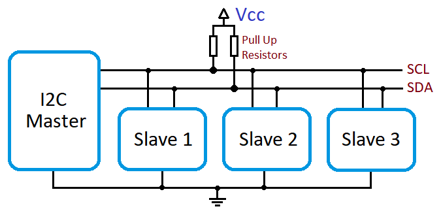
\includegraphics[scale=0.5]{i2c.png}
	\caption{Diagrama del bus I2C}
\end{figure}

\subsection*{Bus SPI}
\begin{itemize}
	
	\item Bus serial de comunicación de tipo maestro-esclavo.
	
	\item Líneas de entrada al esclavo (MOSI) y salida al esclavo (MISO), línea de reloj (SCLK).
	
	\item Línea de selección del chip (SS).
	
\end{itemize}

\begin{figure}[htb]
	\centering
	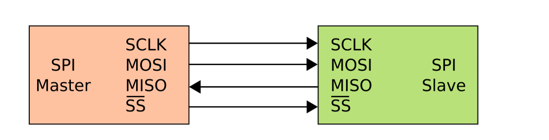
\includegraphics[scale=0.5]{spi.png}
	\caption{Diagrama del bus SPI}
\end{figure}

\subsection*{MPU-6050}
\begin{itemize}
	
	\item Giroscopio de vibración de Coriolis y acelerómetro de 3 ejes.
	
	\item Procesador de movimiento digital (DMP) que mide la orientación del sensor en tres ejes.
	
	\item Buffer FIFO interno.
	
	\item Filtro paso bajo.
	
	\item Comunicación por medio del bus I²C de hasta 400 KHz.
	
	\item Solo puede tomar las direcciones 0x68 y 0x69.
	
\end{itemize}

\begin{figure}[htb]
	\centering
	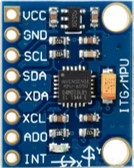
\includegraphics[scale=0.5]{mpu6050.jpg}
	\caption{Sensor inercial MPU6050}
\end{figure}

\subsection*{MPU-9250}
\begin{itemize}
	
	\item Giroscopio de vibración de Coriolis y acelerómetro de 3 ejes.
	
	\item Procesador de movimiento digital (DMP) que mide la orientación del sensor en tres ejes.
	
	\item Buffer FIFO interno.
	
	\item Filtro paso bajo.
	
	\item Comunicación por medio del bus SPI de hasta 10 MHz. \newline\newline
	
\end{itemize}

\begin{figure}[htb]
	\centering
	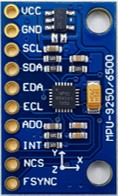
\includegraphics[scale=0.4]{mpu9250.jpg}
	\caption{Sensor inercial MPU9250}
\end{figure}

\subsection*{Sensor flexible capacitivo}
\begin{itemize}
	
	\item Mide el ángulo de torsión al que se somete el sensor en una dirección.
	\item El valor medido es una resistencia variable
	
\end{itemize}

\begin{figure}[htb]
	\centering
	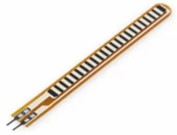
\includegraphics[scale=0.6]{flexsensor.jpg}
	\caption{Sensor flexible capacitivo}
\end{figure}

\subsection*{Convertidor analógico-digital MCP3004}
\begin{itemize}
	
	\item Voltaje de referencia de 2,7 V a 5,5 V
	
\end{itemize}

\begin{figure}[htb]
	\centering
	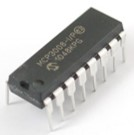
\includegraphics[scale=0.6]{mcp3004.jpg}
	\caption{Convertidor A/D MCP3004}
\end{figure}

\subsection*{Microservomotor posicional}
\begin{itemize}
	
	\item Ángulo de entrada de 0° a 180°
	
	\item Utiliza señales de modulación de ancho de pulso (PWM)
	
	\item Movimiento bidireccional
	
\end{itemize}

\begin{figure}[htb]
	\centering
	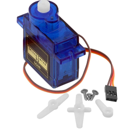
\includegraphics[scale=0.6]{servomotor.png}
	\caption{Microservomotor posicional}
\end{figure}

\newpage
\section*{Propuesta de solución}

\newpage
\section*{Desarrollo}

\subsection*{Sensado}
El algoritmo para obtener los ángulos de inclinación es el que se muestra a continuación.

% Fin del documento
\end{document}